% !TEX root = ../../main.tex

\begin{figure*}[t!]
	\centering
	\begin{subfigure}[t]{0.37\textwidth}
		\centering
		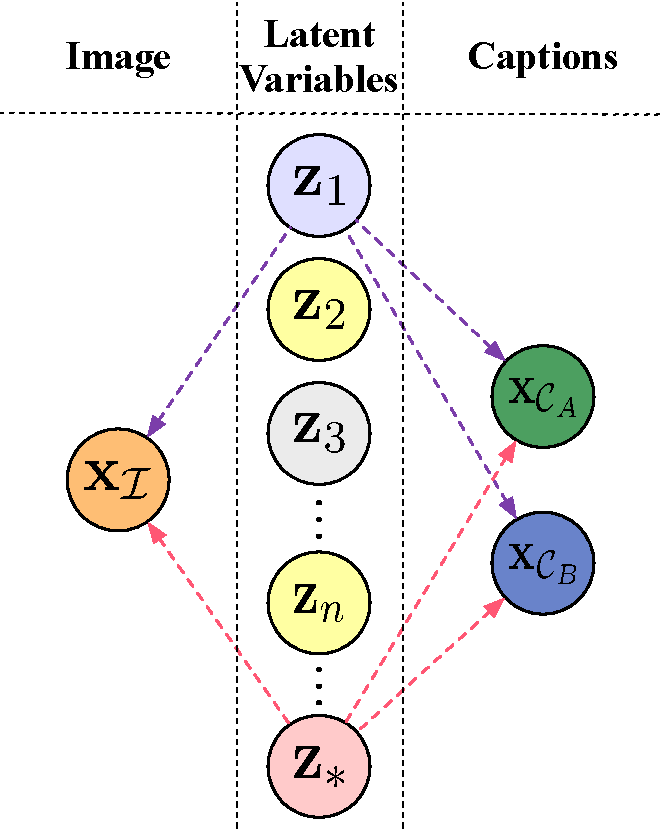
\includegraphics[width=0.75\textwidth]{figures/latent_viz/minimal-shared-representation.pdf}
		\caption{Minimal shared information.}
	\end{subfigure}%
	\qquad
	\begin{subfigure}[t]{0.37\textwidth}
		\centering
		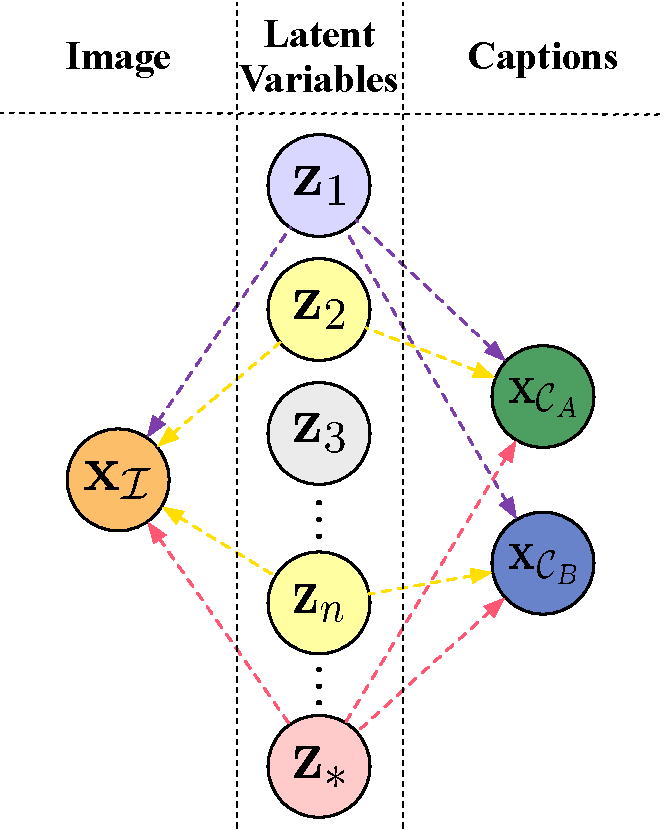
\includegraphics[width=0.75\textwidth]{figures/latent_viz/task-optimal-representation.pdf}
		\caption{Task-optimal information.}
	\end{subfigure}
	\caption{
	Synthetic shortcuts in the context of minimal shared and task-optimal information for vision-language representation learning with multiple captions per image. 
        The purple color represents features shared among the image and all captions (minimal shared information).
        The yellow color represents caption-specific features (unique information).
        The grey color indicates features that are not present in both the image and any of the captions (task-irrelevant information).
        The red color indicates synthetic shortcuts. 
        We demonstrate that while shortcuts exist in both scenarios, minimal shared information also includes information shared among the image and all associated captions, whereas task-optimal information combines both minimal shared information and caption-specific information.
	}
	\label{fig:latent_viz}
\end{figure*} 